\documentclass[../EngineeringJournal_CDavis.tex]{subfiles}

\begin{document}

%%%%%%%%%%%%%%%%%%%%%%%%%%%%%%%%%%%%%%%%%%%%%%%%%%%%%
%%%%%%%%%%%%%%%%%%%%%%%%%%%%%%%%%%%%%%%%%%%%%%%%%%%%%

\chapter[Legacy InterVlan Implementation]{Legacy InterVlan\linebreak[1]
Implementation \hspace*{\fill March 5, 2020}}
\noindent\textbf{{Packet Tracer Lab 14} \hspace*{\fill}{\textbf{CIT 167}}}\linebreak[1]
{{Spring 2020} \hspace*{\fill}{Chaz Davis}}                             
%===================================
%===================================


\hspace{0.2cm}
\begin{tcolorbox}[width=6.3in]
\scriptsize 
Inter Vlan Routing
  \begin{outline}
    \1 router is usually connected to the switch using multiple interfaces.
      \2 One for each VLAN. 
    \1 The interfaces on the router are configured as the default gateways 
      \2 for the VLANs configured on the switch. 
    \1 In this form of inter-VLAN routing 
      \2 router must have as many LAN interfaces as the number of VLANs
  \end{outline}
\normalsize
Scenario:
\scriptsize
- R1 connected to switch ports: G0/0 -> F0/4 (VLAN 10), G0/1 -> F05 (VLAN 30)
- S1 switch ports F0/4 and F0/11 belong to VLAN 10; F0/5 and F0/6 belong to VLAN 30.
\normalsize
Configure the switch:
\scriptsize
\begin{verbatim}
vlan 10		# Create VLAN 10
vlan 30		# Create VLAN 30
interface f0/11
  switchport access vlan 10
interface f0/4
  switchport access vlan 10
interface f0/6
  switchport access vlan 30
interface f0/5
  switchport access vlan 30
  end
\end{verbatim}
\normalsize
Configure the router:
\scriptsize
\begin{verbatim}
interface g0/0
  ip address <default gateway of VLAN10> <subnet-mask>
  no shutdown
interface g0/1
  ip address <default gateway of VLAN 30> <subnet-mask>
  no shutdown
  end
\end{verbatim}
\normalsize
Check routing table with:
\scriptsize
\begin{verbatim}
show ip route
\end{verbatim}
\end{tcolorbox}
\hspace{0.2cm}
\normalsize  
  
\clearpage

%===================================
\mysection{\textbf{Part 1: Configuring and verifying the network}}

\mysubsection{1}{Configuring The Pcs}\\
I setup the Configuration according to the handout. I then, configured the IP
address, default gateways, and subnet masks on each of the PCs.


\begin{figure}[!hbt]\centering
\subfloat[IP config on PC1]{\label{IPC14PC1}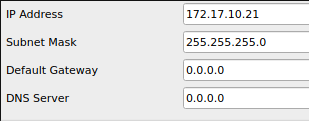
\includegraphics[width=.45\linewidth]{Figures/2020-03-19-184631_309x121_scrot.png}}\hfill
\subfloat[IP Config on PC3]{\label{IPC14PC3}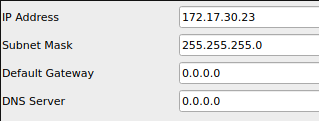
\includegraphics[width=.45\linewidth]{Figures/2020-03-19-184712_319x121_scrot.png}}\par 
\caption{IP Configurations}\label{IPC14}
\end{figure}

\noindent\mysubsection{2}{Configuring The Router and Switch}\\
I Next ran the commands on R1, 
You can see in Fig.~\ref{Net14}~\subref{Net14R1} 
on Pg.~\pageref{Net14}, the results of show ip int brief.
And then the commands on S1, as you can see in
Fig.~\ref{Net14}\subref{Net14Ip1} and Fig.~\ref{Net14}\subref{Net14Vlan1} 
on Pg.~\pageref{Net14}, the results of 
{\scriptsize{\verb$show ip int brief$}\normalsize}  and 
{\scriptsize{\verb$show vlan brief$}\normalsize}  on
switch 1.

I had to go back
and run {\scriptsize{\verb$int g0/1 no shut$}\normalsize} on R1.
As You can see in Fig.~\ref{Net14}\subref{Net14R2}, the output of the
{\scriptsize{\verb$show ip int brief$}\normalsize} 
and the output of {\scriptsize{\verb$show vlan brief$}\normalsize} on S3
in Fig.~\ref{Net14}\subref{Net14Vlan2}
on Pg.~\pageref{Net14}.


\begin{figure}[!hbt]\centering
\subfloat[Show ip int brief on R1]{\label{Net14R1}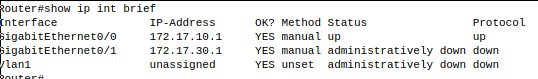
\includegraphics[width=.45\linewidth]{Figures/2020-03-19-184832_538x79_scrot.png}}\hfill
\subfloat[show ip int brief on S1]{\label{Net14Ip1}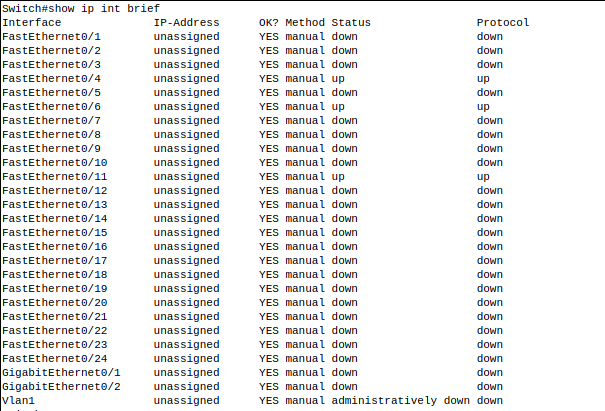
\includegraphics[width=.45\linewidth]{Figures/2020-03-19-185004_605x411_scrot.png}}\par
\subfloat[show vlan brief on S1]{\label{Net14Vlan1}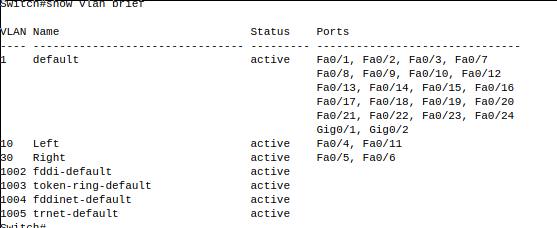
\includegraphics[width=.45\linewidth]{Figures/2020-03-19-185014_557x228_scrot.png}}\par
\subfloat[show ip in brief on R1 after command]{\label{Net14R2}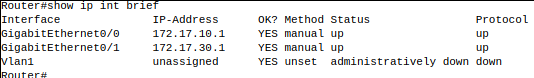
\includegraphics[width=.45\linewidth]{Figures/2020-03-19-185250_534x78_scrot.png}}\hfill
\subfloat[show ip int brief on S1 after command]{\label{Net14Vlan2}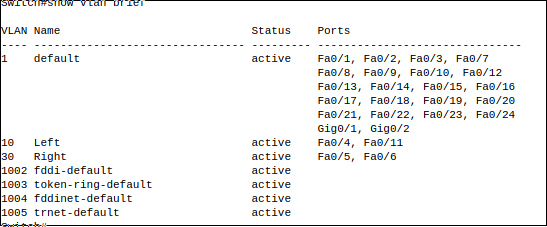
\includegraphics[width=.45\linewidth]{Figures/2020-03-19-185333_547x227_scrot.png}}\par
\caption{Configuration of R1 and S1}\label{Net14}
\end{figure}

\clearpage

\noindent\mysubsection{3}{Checking the Connections}\\
After that I was able to successfully ping from PC1 to PC3.


\begin{figure}[!hbt]\centering
\subfloat[Pinging from PC1 to PC3]{\label{success14ping}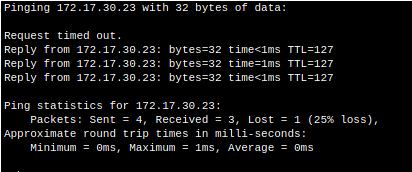
\includegraphics[width=.45\linewidth]{Figures/2020-03-08-194333_412x172_scrot.png}}\par
\subfloat[Successful network architecture]{\label{success14arch}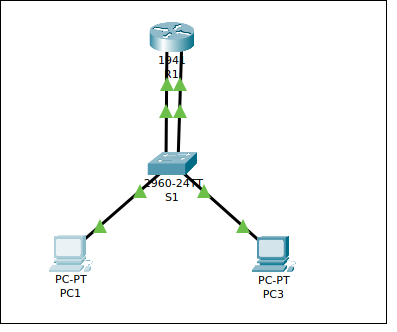
\includegraphics[width=.45\linewidth]{Figures/2020-03-08-194344_397x332_scrot.png}}\par
\caption{Successful Lab layout}\label{success14}
\end{figure}

%===================================

\end{document}
